%----------------------------------------------------------------------------------------
%	PACKAGES AND OTHER DOCUMENT CONFIGURATIONS
%----------------------------------------------------------------------------------------

\documentclass{article}

\usepackage{fancyhdr} % Required for custom headers
\usepackage{lastpage} % Required to determine the last page for the footer
\usepackage{extramarks} % Required for headers and footers
\usepackage[usenames,dvipsnames]{color} % Required for custom colors
\usepackage{graphicx} % Required to insert images
\usepackage{listings} % Required for insertion of code
\usepackage{courier} % Required for the courier font
\usepackage{lipsum} % Used for inserting dummy 'Lorem ipsum' text into the template
\usepackage[T1]{fontenc}
\usepackage{titlesec, blindtext, color}
\usepackage{natbib}
\usepackage{dirtree}
\usepackage{multirow}
\usepackage{booktabs}
\usepackage{array, tabularx, caption, boldline}
\usepackage{beramono}
\usepackage{hyperref}
\usepackage[section]{placeins}

% Margins
\topmargin=-0.45in
\evensidemargin=0in
\oddsidemargin=0in
\textwidth=6.5in
\textheight=9.0in
\headsep=0.25in

\linespread{1.1} % Line spacing

% Set up the header and footer
\pagestyle{fancy}
\lhead{\HeaderTitle} % Top left header
%\chead{\Title} % Top center head
\rhead{\firstxmark} % Top right header
\lfoot{\lastxmark} % Bottom left footer
\cfoot{} % Bottom center footer
\rfoot{Page\ \thepage\ of\ \protect\pageref{LastPage}} % Bottom right footer
\renewcommand\headrulewidth{0.4pt} % Size of the header rule
\renewcommand\footrulewidth{0.4pt} % Size of the footer rule

\setlength\parindent{0pt} % Removes all indentation from paragraphs

%----------------------------------------------------------------------------------------
%	CODE INCLUSION CONFIGURATION
%----------------------------------------------------------------------------------------

\definecolor{codegreen}{rgb}{0,0.6,0}
\definecolor{codegray}{rgb}{0.5,0.5,0.5}
\definecolor{codepurple}{rgb}{0.58,0,0.82}
\definecolor{backcolour}{rgb}{0.95,0.95,0.92}

\lstdefinestyle{codestyle}{
	basicstyle=\fontfamily{fvm}\selectfont\footnotesize,
    backgroundcolor=\color{backcolour},   
    commentstyle=\color{codegreen},
    keywordstyle=\color{magenta},
    numberstyle=\tiny\color{codegray},
    stringstyle=\color{codepurple},
%    basicstyle=\footnotesize,
    breakatwhitespace=false,         
    breaklines=true,                 
    captionpos=b,                    
    keepspaces=true,                 
    numbers=left,                    
    numbersep=5pt,                  
    showspaces=false,                
    showstringspaces=false,
    showtabs=false,                  
    tabsize=2
}

\lstset{style=codestyle}

%----------------------------------------------------------------------------------------
%	DOCUMENT STRUCTURE COMMANDS
%	Skip this unless you know what you're doing
%----------------------------------------------------------------------------------------

\titlespacing*{\section}
{0pt}{24pt plus 4pt minus 0pt}{12pt plus 2pt minus 0pt}
\titlespacing*{\subsection}
{0pt}{12pt plus 4pt minus 0pt}{1pt plus 0pt minus 0pt}

\hyphenation{DELPHIN}

\hypersetup{
    colorlinks=true,
    linkcolor=blue,
    filecolor=magenta,      
    urlcolor=cyan,
}

%----------------------------------------------------------------------------------------
%	NAME AND CLASS SECTION
%----------------------------------------------------------------------------------------

\newcommand{\Title}{Monte-Carlo simulations with DELPHIN 5.8 \\using Python package SHARK}
\newcommand{\SubTitle}{A Python tutorial}
\newcommand{\AuthorName}{Astrid Tijskens}
\newcommand{\AuthorEmail}{astrid.tijskens@kuleuven.be}
\newcommand{\HeaderTitle}{Monte-Carlo simulations with DELPHIN 5.8 using SHARK}

\newcommand{\file}[1]{{\small\texttt{#1}}}
\newcommand{\code}[1]{{\small\texttt{#1}}}

\setlength{\extrarowheight}{0.3cm}

%----------------------------------------------------------------------------------------
%	TITLE PAGE
%----------------------------------------------------------------------------------------

\title{
%\vspace{1cm}
\textmd{\textbf{\Title}}\\
\normalsize\vspace{0.3cm}
\large{\SubTitle}
\vspace{1cm}
}

\author{\textbf{\AuthorName}\\
\small{\AuthorEmail}
}
\date{05-12-2017}

%----------------------------------------------------------------------------------------
%	START DOCUMENT
%----------------------------------------------------------------------------------------

\begin{document}

\maketitle

%\setcounter{tocdepth}{1} % Uncomment this line if you don't want subsections listed in the ToC
\tableofcontents
\newpage

\section{Introduction}
To facilitate probabilistic Monte-Carlo simulations with DELPHIN 5.8, a Python package called 'SHARK' was developed. SHARK allows the user to:
\begin{itemize}
	\item Create a sampling scheme from given parameter distributions
	\item Automatically change parameter values in existing DELPHIN project files and save these as new DELPHIN project files
	\item Automatically run the newly created DELHIN project files
	\item Post-process the simulation output using different damage prediction models
\end{itemize}
SHARK is able to automatically recognise which parameters need to be edited by which values. For this to work, however, some formatting rules need to be followed. This tutorial describes step-by-step how to set up the project correctly and how to use SHARK. The general work flow, based on the probabilistic methodology developed by \citet{VanGelder2014a}, is as follows:
\begin{enumerate}
	\item Create one DELPHIN project file for each design options
	\item Generate sampling scheme based on the given parameters and parameter distributions
	\item Generate DELPHIN project files based on the design options and sampling scheme
	\item Run the simulations
	\item Post-process the simulation output 
\end{enumerate}
These different steps will be explained in the following sections.

\subsection{Installing Python and SHARK}
The best way to install Python is via Anaconda. Go to \url{https://www.anaconda.com/download}, download the Python 3.6 version for your machine and install. After installing, open an Anaconda Command Prompt and type:
\begin{lstlisting}[language=command.com]
python -V
\end{lstlisting}
This should return the following (or something similar):
\begin{lstlisting}[language=command.com]
Python 3.6.2 :: Anaconda custom (64-bit)
\end{lstlisting}
Once Python is installed, you can install SHARK to following way. Save \file{SHARK-0.1.0.zip} somewhere on your computer. Go to the folder \file{\textasciitilde{}\textbackslash{}SHARK-0.1.0\textbackslash{}shark\textbackslash{}data\textbackslash{}} and open \file{dir\_ext\_clim.txt}. Change the path you see here to the directory where you store your climate data and save the file. \\
Open an Anaconda Command Prompt and change the working directory to the path of \file{SHARK-0.1.0.zip} by typing the following (replace \code{\textasciitilde{}\textbackslash{}path} by the path where you extracted \file{SHARK-0.1.0.zip}) :
\begin{lstlisting}[language=python]
cd ~\path\SHARK-0.1.0
\end{lstlisting}
Next, type the following:
\begin{lstlisting}[language=command.com]
python setup.py install
\end{lstlisting}
If you are asked to install dependent packages, do so. If no errors come up, SHARK should be installed. You can check this by going to \file{C:\textbackslash{}Users\textbackslash{}YourName\textbackslash{}Anaconda3\textbackslash{}Lib\textbackslash{}site-packages} or by typing the following:
\begin{lstlisting}[language=command.com]
conda list
\end{lstlisting}
If SHARK is listed, it was installed correctly and you can proceed using SHARK.

\subsection{SHARK updates and reporting bugs}
SHARK is uploaded on \url{https://github.com/astridtijskens/Shark}. New versions or updates will become available here. If you encounter a bug or an issue, this can be reported on \url{https://github.com/astridtijskens/Shark/issues}.

\section{Creating DELPHIN project files}
A probabilistic DELPHIN project has a specific folder structure. The example accompanied by this tutorial has the same folder structure. This structure should be kept as is and not changed. \vspace{0.3cm}

\begin{minipage}{0.75\linewidth}
	\dirtree{%
	.1 'Project~name'~(e.g.~Example). 
	.2 Delphin~files. 
	.3 Materials. 
	.4 'material\_file.m6'~(e.g.~brick\_001.m6). 
	.4 ...~. 
	.3 Originals. 
	.4 'design\_option.dpj'~(e.g.~Option\_000.dpj). 
	.4 ...~. 
	.2 Sampling~scheme. 
	.2 config.py. 
	.2 run.py. 
	.2 postprocess.py. 
	}
\end{minipage}
\vspace{0.3cm}\\
Once the folder structure is created, the first step is to create one DELPHIN project file for each design option included in the probabilistic analysis. As this is very project specific, this step is not automated but needs to be done manually. In this tutorial, an external wall with internal insulation is studied and seven design options are included: a reference wall, without insulation (\file{Option\_000.dpj)}, a wall with 5, 10 and 20\,cm XPS insulation (\file{Option\_001.dpj}, \file{Option\_002.dpj}, \file{Option\_003.dpj}) and a wall with 5, 10 and 20\,cm CaSi insulation (\file{Option\_004.dpj}, \file{Option\_005.dpj}, \file{Option\_006.dpj}). These DELPHIN project files are created as usual. For SHARK to work however, some formatting rules need to be followed.

\subsection{Automatically changing materials}
If you want to include different materials in the probabilistic assessment, e.g. different brick types for the masonry wall, you need to insert all the different materials into the DELPHIN project file, but assign only one of them to the construction, as shown in figure \ref{fig:materials}. Which one you assign does not matter. All materials need to have the same name, combined with a number or letter, e.g. `Brick1', `Brick2', `Brick3' or `insulation\_A', `insulation\_B', `insulation\_C'. Furthermore, these materials should be saved in the 'Materials' folder. 

\begin{figure}
	\centering
	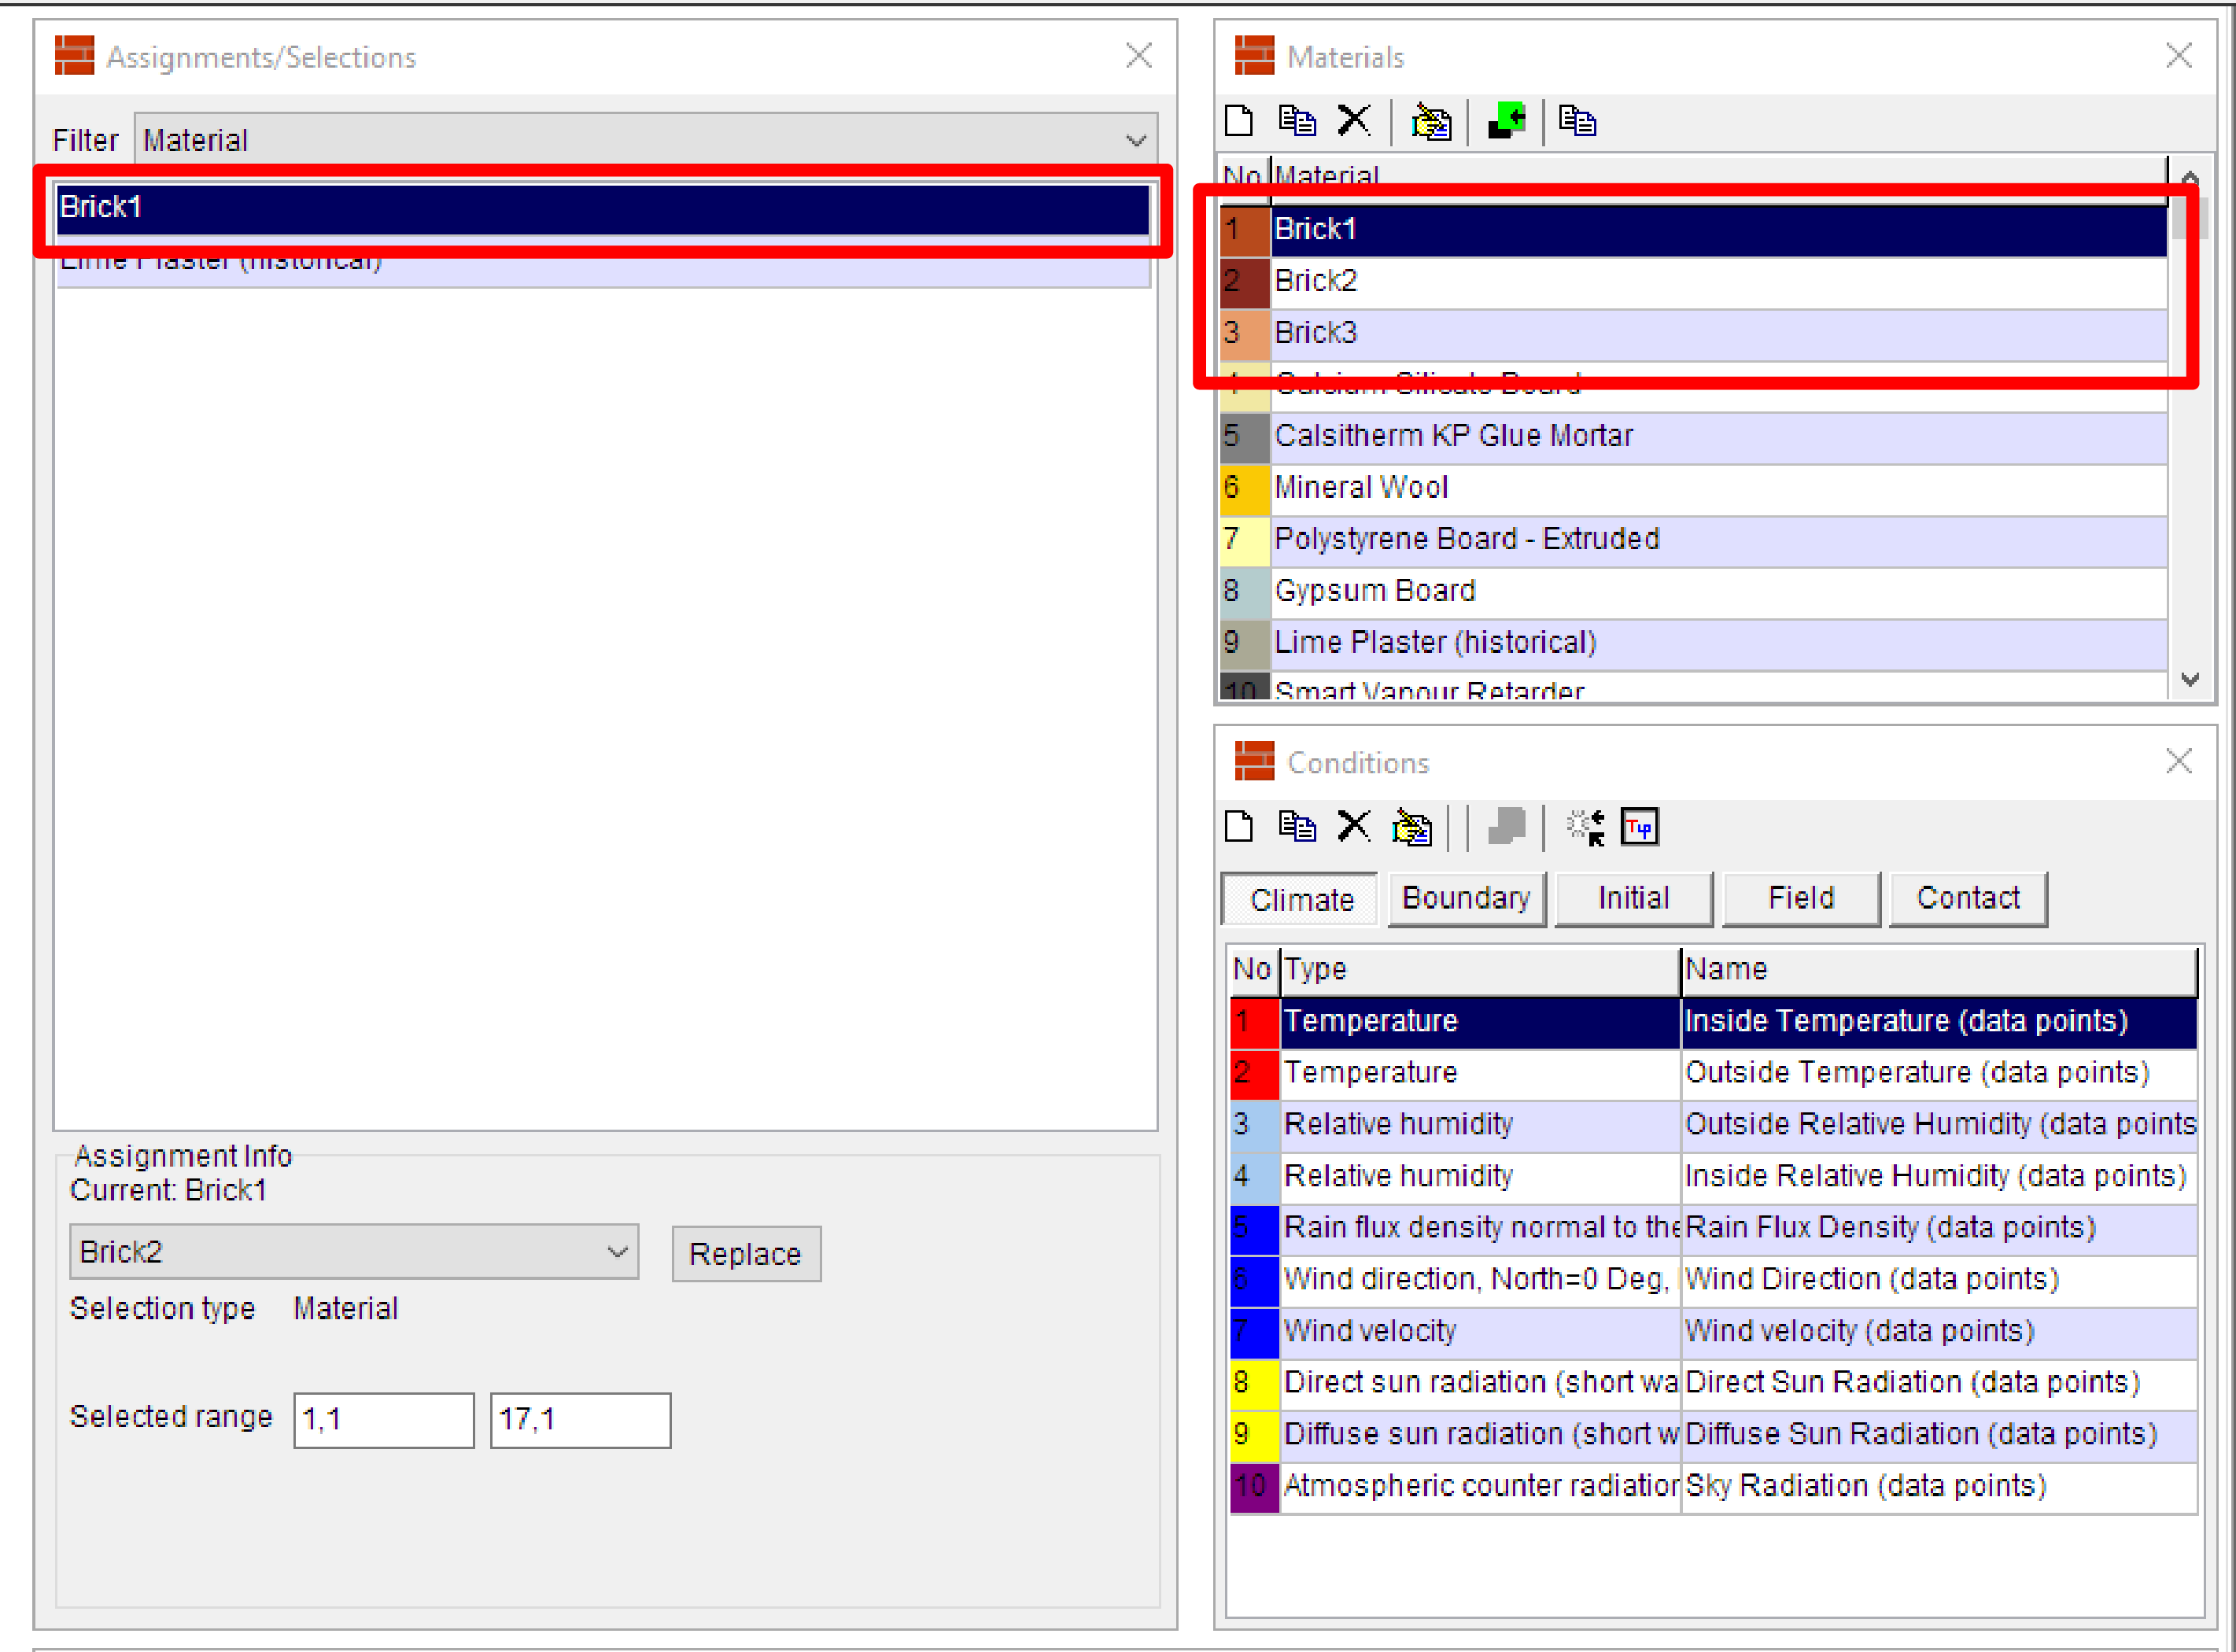
\includegraphics[width=0.75\textwidth]{./Figures/Materials}
	\caption{Three brick materials are imported into the project file, but only one is assigned to the construction.}
	\label{fig:materials}
\end{figure}

To insert a material in a DELPHIN file from an external source (not the DELPHIN material database), right click in the Materials window and click on 'insert from external file'. So can also export materials from DELPHIN (e.g. after editing a material from the database) by right clicking on the material and selecting 'Export material file'.\\
\vspace{0cm}\\
Note: Although it would technically be possible to change the material parameters of a specific material file, instead of using different material files, this is not supported by SHARK. This is because the parameters of a material often are not independent of each other, thus changing only one parameter might result in an unrealistic material.

\subsection{Automatically changing dimensions of a building component}
It is possible to automatically change the dimensions of a building component, e.g. the brick wall thickness. For this to work, the DELPHIN geometry should be discretised (as usual), except for the building component of which you want to change the dimensions. This is shown in figure \ref{fig:dimension}. If you want to have assign outputs within the building component of which you want to change the dimensions, this is possible by only discretising the part where you want to have an output. In the example, we want to have an output at 0.5\,cm from the exterior surface (i.e. to evaluate the frost damage risk) and at 5\,cm from the interface between masonry and plaster or insulation system (i.e. to evaluate the damage risk for wooden beam ends). Hence, the first 0.5\,cm and last 5\,cm are discretised, the part in between is not. SHARK will automatically change the dimensions of this column according to the sampled dimension values (see section \ref{sec:sample+variation}) and subsequently discretise this column.

\begin{figure}
	\centering
	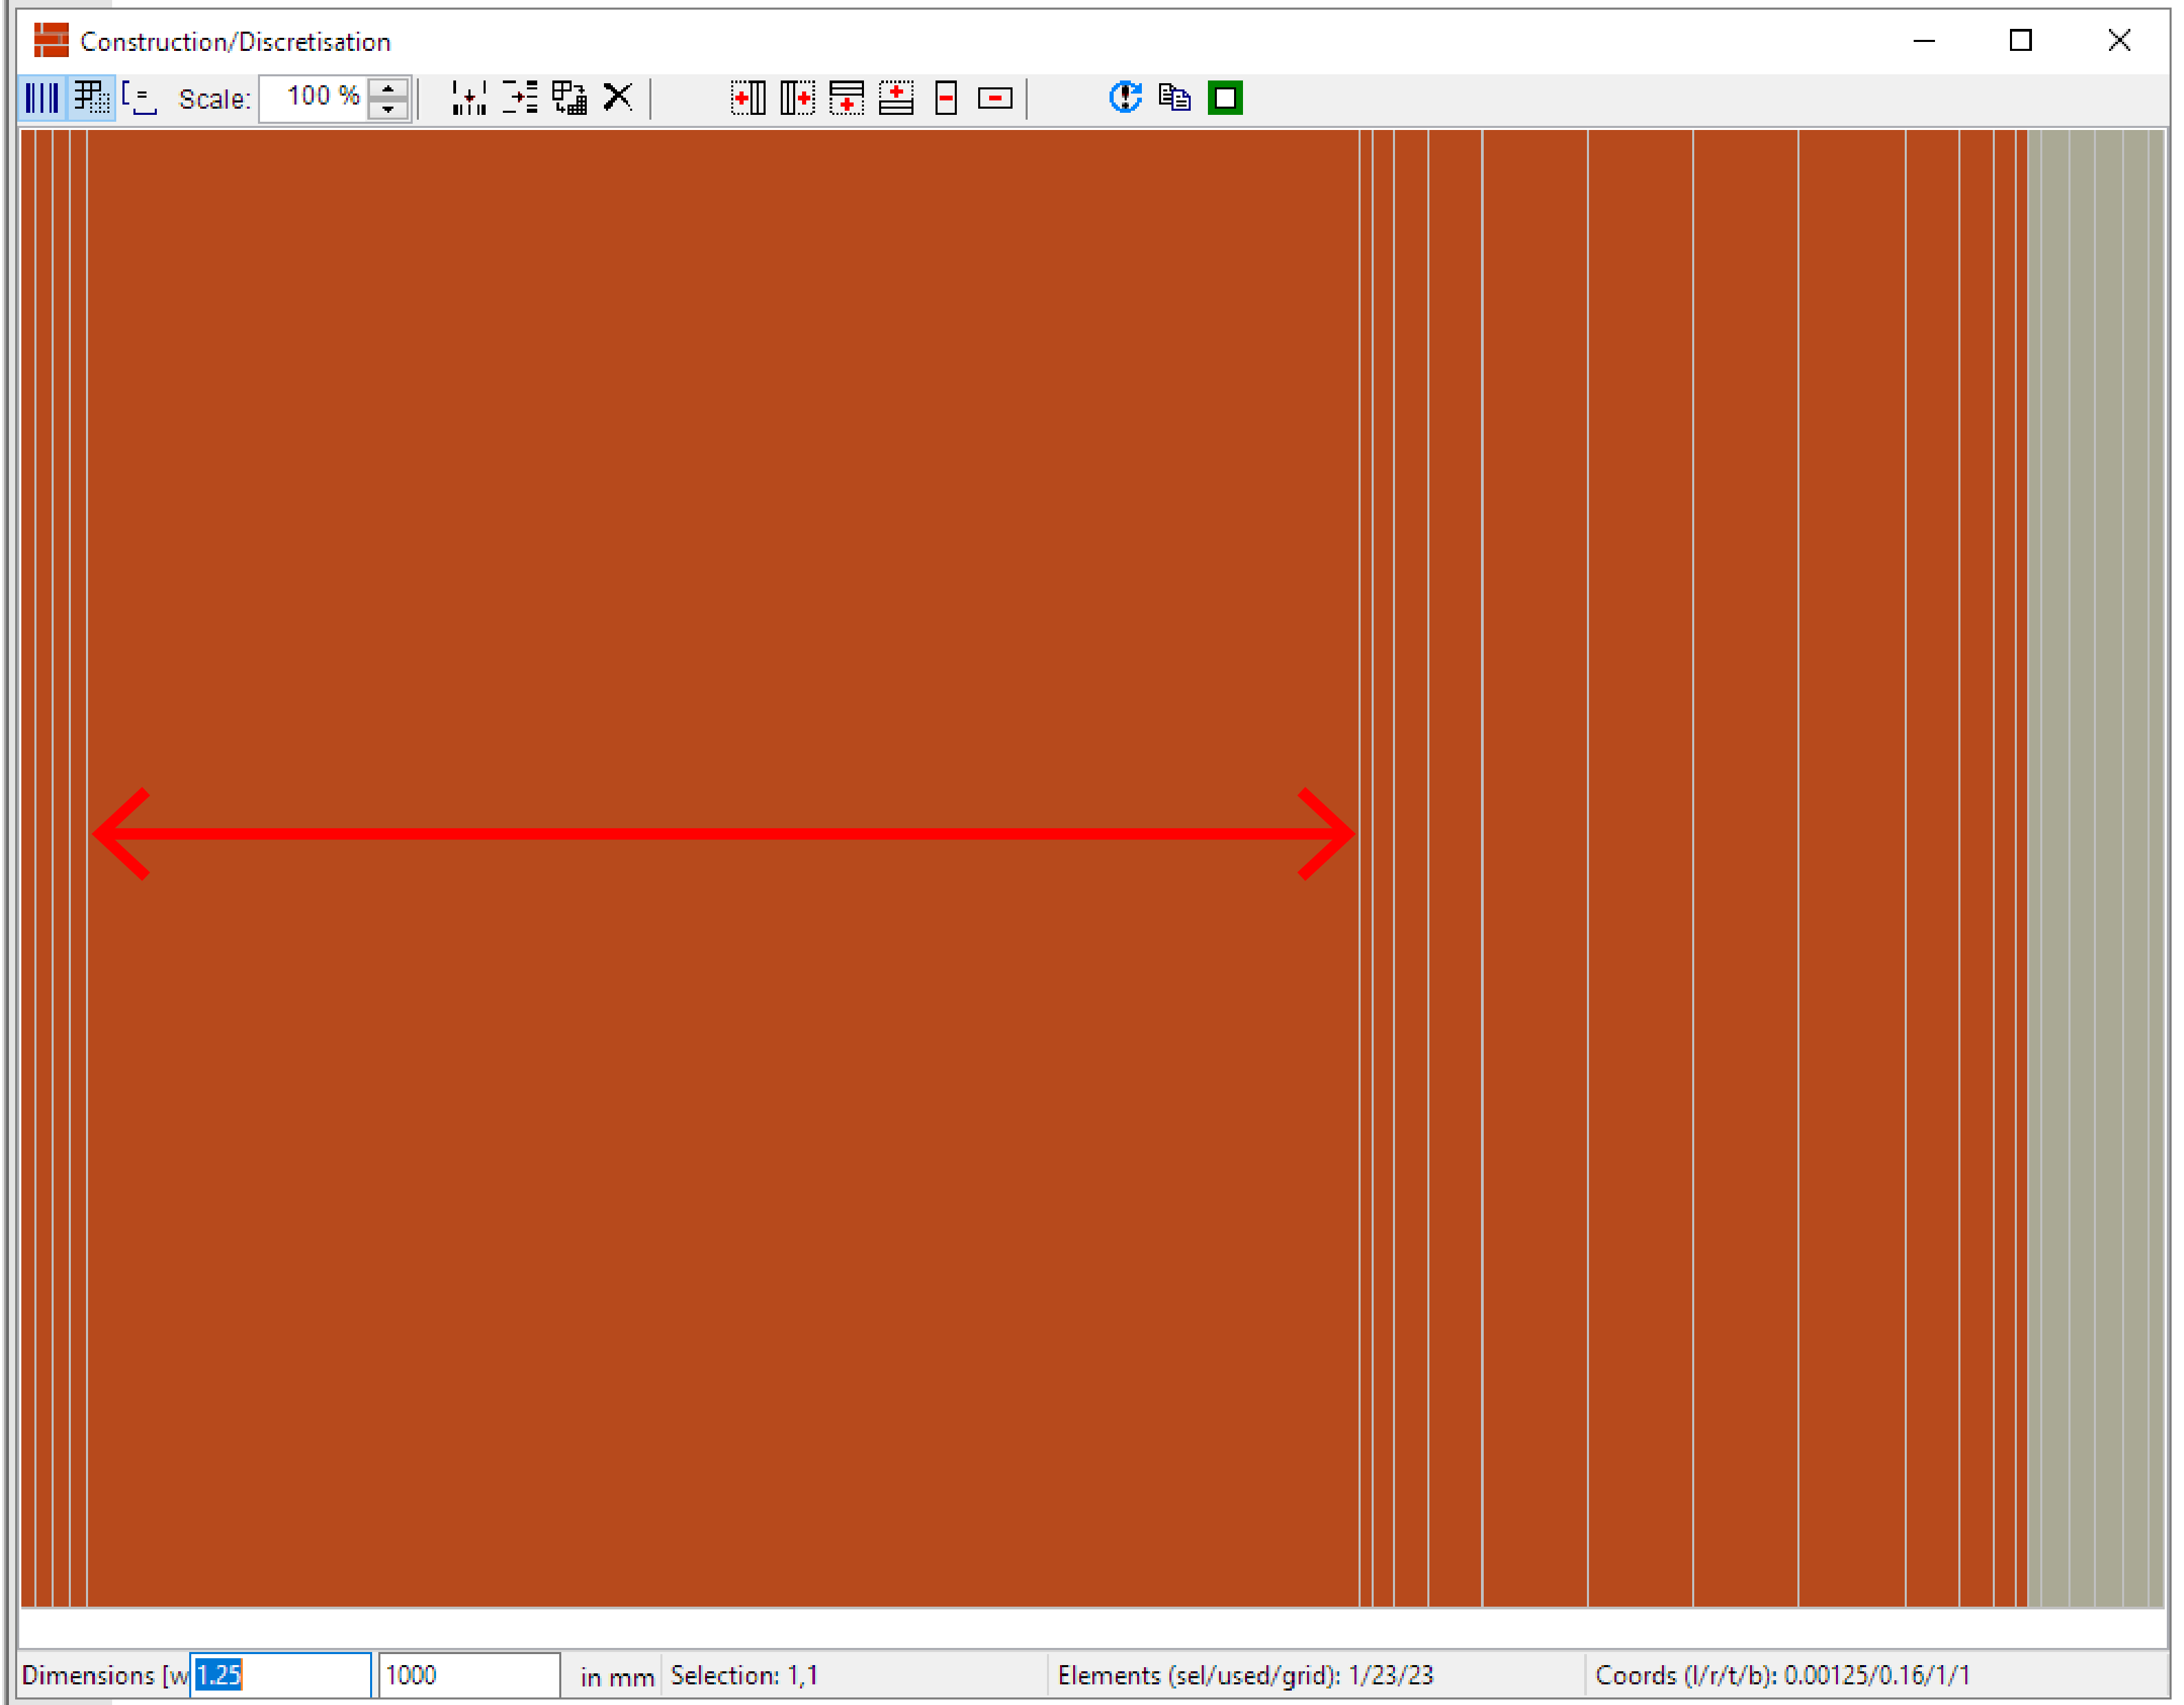
\includegraphics[width=0.8\textwidth]{./Figures/Dimension}
	\caption{Part of the brick wall component is not discretised. The dimension of this column will be edited by SHARK, after which the column is automatically discretised.}
	\label{fig:dimension}
\end{figure}

\subsection{Automatically changing interior and exterior climate}
The interior and exterior climate can automatically be changed if the climate conditions and boundary conditions are named correctly. The name of the climate conditions of the interior temperature and relative humidity or vapour pressure should contain the word 'inside'; the name of the climate conditions for the exterior temperature and relative humidity should contain the word 'outside'. Both upper and lower case (or a combination) are allowed. All other exterior climate conditions (rain, wind velocity, wind direction, direct radiation, diffuse radiation, atmospheric radiation) can be named arbitrarily. The same rules apply for the boundary conditions, as shown in figure \ref{fig:climatecond}.

\begin{figure}
	\centering
	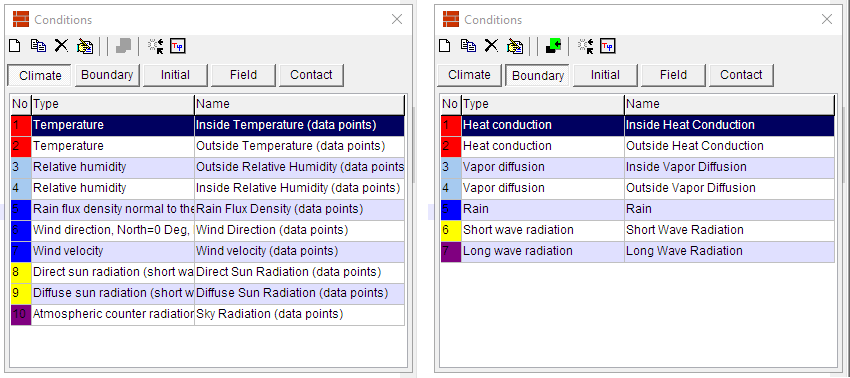
\includegraphics[width=0.8\textwidth]{./Figures/ClimateBCcond}
	\caption{Example of how to name the interior and exterior climate and boundary conditions.}
	\label{fig:climatecond}
\end{figure}

\subsection{Assigning the outputs}
The outputs are assigned as usual. No formatting rules apply for the names of the output files. For clarity, however, it is recommended not to include any numbering in the file names, as SHARK will add a numbering as well. \\
\vspace{0cm}\\
Note: Assign only the outputs you really need for post-processing or damage prediction. Writing the output during the simulations is slow (even when you have an SSD). For computers with more than 8 CPU's, the bottleneck in the simulations are not the actual calculations, but writing the output to the disk. Hence, reducing the amount of output might reduce the total simulation time.

\FloatBarrier

\section{Creating a sampling scheme and generating variation DELPHIN project files}
\label{sec:sample+variation}
This step is performed by the script \file{config.py}. Before SHARK can do its work, you need to define the parameter distributions and all the other variables needed for the probabilistic assessment.\\
First, you need to define the interior climate model and the scenario layer, as shown in listing \ref{list:scenario}. The scenario layer always defines the interior climate, based on the selected model. Currently, two European Standards are implemented: EN\,15026 \citeyearpar{EN15026} and EN\,13788 \citeyearpar{EN13788}. Table \ref{tab:scenario} shows which values should be entered for which model. Note that it is possible to enter only one value or only some of the possible values (e.g. for EN\,13788 \code{[2,3]} and for EN\,15026 \code{['a']} are both valid entries). It is not possible to leave out the scenario layer, you should always select at least one scenario. It is also not possible to combine the two interior climate models in the same project.

\begin{minipage}{\linewidth}
\begin{lstlisting}[language=Python, caption=Define the scenario layer.]
# Scenario layer - scenario's
interior_climate_type = 'EN15026' # Use 'EN15026' or 'EN13788'
scenario = {'parameter':'int climate', 'value':['a','b']}
\end{lstlisting}
\label{list:scenario}
\end{minipage}

\begin{table}[h]
  \centering
  \caption{The possible entries for \code{value} in the DataFrame \code{senario} for the available interior climate models.}
  \label{tab:scenario}
  \begin{tabularx}{0.38\textwidth}{>{\hsize=.6\hsize\raggedright\arraybackslash}X|>{\hsize=1.4\hsize\raggedright\arraybackslash}X}
	\textbf{model}	& \textbf{\code{value}} \\
	\hlineB{1.2}
    EN 15026		& \code{[`a', `b']} or \code{[1, 2]}\\
    EN 13788		& \code{[1, 2, 3, 4]} \\
    \end{tabularx}%
\end{table}%

Next, the parameter distributions of the uncertainty layer need to be defined, as shown in listing \ref{list:distr}. The distributions are combined in a DataFrame with three columns: \code{parameter}, \code{type} and \code{value}. Table \ref{tab:distrparam} shows the possible values for \code{parameter} and their meaning and Table \ref{tab:distrtypeval} shows the possible distribution types and their respective value formatting. If you want to change the material of a building component, the parameter name should consist of the word \code{material} and the material name you gave to it in DELPHIN. In the example, we want to change the material of the masonry wall. We gave the materials the name \code{Brick1}, \code{Brick2} and \code{Brick3} and assigned \code{Brick1} to the geometry. Hence, the parameter for changing the material is \code{brick material}, as shown on line 11-13 of listing \ref{list:distr}. The command is insensitive for the word order the case of the material name. If you want to change the the dimensions of a building component, you do not need to add the material name. However, this is recommended for clarity. 

\begin{minipage}{\linewidth}
\begin{lstlisting}[language=Python, caption=Define the parameter distributions.]
# Uncertainty layer - Parameter distributions
distributions = pd.DataFrame([{'parameter':'solar absorption', 
																		'type':'uniform',   
																	 'value':[0.4,0.8]},
                              {'parameter':'ext climate',
                                		'type':'discrete',  
                                	 'value': ['Oostende','Gent','StHubert','Gaasbeek']},
                              {'parameter':'exterior heat transfer coefficient slope',
                                		'type':'uniform',  
                                	 'value':[1,8]},
                              {'parameter':'brick material',
                                		'type':'discrete',   
                                	 'value':['Brick1','Brick2','Brick3']},
                              {'parameter':'scale factor catch ratio',
                                		'type':'uniform',    
                                	 'value':[0,1.5]},
                              {'parameter':'wall orientation', 
                                		'type':'uniform',  
                                	 'value':[0,360]},
                              {'parameter':'start year',  
                                		'type':'discrete',   
                                	 'value':24},
                              {'parameter':'brick dimension',
                                		'type':'uniform',    
                                	 'value':[0.15,0.5]},
                              ])
\end{lstlisting}
\label{list:distr}
\end{minipage}

\begin{table}
  \centering
  \caption{The possible entries for \code{parameter} in the DataFrame \code{distributions}.}
  \label{tab:distrparam}
  \begin{tabularx}{1\textwidth}{>{\hsize=.5\hsize\raggedright\arraybackslash}X|>{\hsize=1.5\hsize\raggedright\arraybackslash}X}
	\textbf{Parameter}										& \textbf{Meaning} \\
	\hlineB{1.2}
    \code{wall orientation}									& the orientation of the wall \\
    \code{wall inclination	}								& the inclination of the wall \\
    \code{exterior heat transfer coefficient}				& {the heat transfer coefficient, defined by the exterior boundary condition, type `heat conduction', kind `exchange coefficient'} \\
    \code{exterior heat transfer coefficient slope}			& {the heat transfer coefficient slope, defined by the exterior boundary condition, type `heat conduction', kind `boundary layer'} \\
    \code{interior vapour diffusion transfer coefficient}	& {the vapour diffusion transfer coefficient, defined by the interior boundary condition, type `vapour diffusion', kind `exchange coefficient'} \\
    \code{exterior vapour diffusion transfer coefficient}	& {the vapour diffusion transfer coefficient, defined by the exterior boundary condition, type `vapour diffusion', kind `exchange coefficient'} \\
    \code{exterior vapour diffusion transfer coefficient slope}	& {the vapour diffusion transfer coefficient slope, defined by the exterior boundary condition, type `heat conduction', kind `boundary layer'} \\
    \code{solar absorption}									& {the solar absorption, defined by the exterior boundary condition, type `short wave radiation', kind `direct sun radiation model'} \\
    \code{scale factor catch ratio}							& {the rain exposure coefficient, defined by the exterior boundary condition, type `rain', kind `imposed flux'} \\
    \code{ext climate}										& the exterior climate location \\
    \code{start year}										& {the start year for the exterior climate (only meaningful if using climate data with more than one year}  \\
	\code{$*$ material}										& the material that needs to be changed \\
	\code{$*$ dimension}									& the building component of which the dimension need to be changed \\
	\multicolumn{2}{l}{\footnotesize Replace * by material name, e.g. `brick' }\\
    \end{tabularx}%
\end{table}%

\begin{table}
  \centering
  \caption{The possible entries for \code{value} in the DataFrame \code{distributions}.}
  \label{tab:distrtypeval}
  \begin{tabularx}{1\textwidth}{>{\hsize=.5\hsize\raggedright\arraybackslash}X|>{\hsize=1.5\hsize\raggedright\arraybackslash}X}
	\textbf{Distribution type}	& \textbf{Distribution parameter values} \\
	\hlineB{1.2}
    \code{uniform}				& \code{[}\textit{minimum value}\code{,} \textit{maximum value}\code{]} \\
    \code{normal}				& \code{[}\textit{mean}\code{,} \textit{standard deviation}\code{]} \\
    \code{discrete}				& \code{[}\textit{value 1}\code{,} \textit{value 2}\code{,} \textit{value 3}\code{,} ...\code{]} or \textit{maximum value} \\
    \end{tabularx}%
\end{table}%

Next, you need to provide SHARK with the details about the sampling scheme, as shown in listing \ref{list:sampling}. Currently, there are two possibilities for \code{sampling\_strategy}:

\begin{enumerate}
	\item \code{'load'}: an existing raw sampling design (values not yet converted to parameter distributions) is loaded from the folder \file{Sampling scheme}. SHARK converts the raw sampling design to a sampling scheme. The variables \code{samples\_per\_set} and \code{sets} are ignored, you can set both to \code{Null}.
	\item \code{'sobol'}: a new sampling design is created, using the scrambled sobol sampling strategy. Subsequently, this sampling design is converted to a sampling scheme. The variables \code{samples\_per\_set} and \code{sets} are required.
\end{enumerate}

The final result is the same: a sampling scheme that will be used for the probabilistic assessment. If you don't have an existing raw sampling design, use \code{'sobol'}. The variable \code{samples\_per\_set} defines how many samples are created per set. The variable \code{sets} defines how many sets are created. Remember that we defined two scenario's in the scenario layer. The total number of samples will be \textit{number of scenario's} x \code{samples\_per\_set} x \code{sets}. For the example, this is 2 x 18 x 3 = 108~samples.

\begin{minipage}{\linewidth}
\begin{lstlisting}[language=Python, caption=Enter the sampling scheme details.]
# Sampling details
sampling_strategy = 'sobol'
samples_per_set = 18
sets = 3
\end{lstlisting}
\label{list:extclim}
\end{minipage}

Next, you need to define some parameters about the exterior climate, as shown in \ref{list:extclim}. You have mainly two possibilities for the exterior climate: you use yearly cyclic data (e.g. the climata data provided by DELPHIN), or you use climata data that consists of multiple years (e.g. the Climate for Culture data). In the latter case, you need to define how many years the simulation runs via the variable \code{number\_of\_years}. Note that this should be a whole number, even if your simulation does not run for full years. In the example the simulation starts in September and runs for 6 years and four months; hence, \code{number\_of\_years} is 7 as 7 years of data will be used. Furthermore, you need to define weather you want to use wind driven rain via the variable \code{simulate\_wdrain}. If this is the case, it is important that you used the climate condition type \textit{Rain flux density normal to the wall surface} and the boundary condition type \textit{Rain} of kind \textit{Imposed flux}. SHARK has it's own rain model, based on \cite{Blocken2004}, as the rain model of DELPHIN is not very accurate. SHARK will automatically calculate the rain flux based on the provided exterior climates and the wall orientation. If you do not wish to include wind-driven rain, set \code{simulate\_wdrain} to \code{False}. This is usually not recommended, although it can be usefull in some cases (e.g. in case of a wall with fa\c{c}ade cladding).

\begin{minipage}{\linewidth}
\begin{lstlisting}[language=Python, caption=Provide the exterior climate details.]
# Climate info
number_of_years = 7
simulate_wdrain = True 
\end{lstlisting}
\label{list:sampling}
\end{minipage}

Finally, you need to tell SHARK of which building component you want to change the dimensions, as shown in \ref{list:buildcomp}. The variable \code{buildcomp} is a list with two elements: the first element is the first column or row of the building component in DELPHIN; the second element is the last column or row of the building component. You can find the column/row numbering in DELPHIN by selecting a cell; at the bottom of the Construction window, you will see \textit{Selection: x,y}: \textit{x} is the column, \textit{y} is the row. The variable \code{buildcomp\_elem} defines which column/row need to be changed in dimension (this column/row should not be discretised!). The variable \code{dir\_cr} tells SHARK whether it is a column (\code{'column'}) or a row (\code{'row'}).

\begin{minipage}{\linewidth}
\begin{lstlisting}[language=Python, caption=Define the building component of which the dimensions need to be changed.]
# Change dimensions of building component
buildcomp = [1,17]
buildcomp_elem = 5
dir_cr = 'column'
\end{lstlisting}
\label{list:buildcomp}
\end{minipage}

The rest of the script \file{config.py} should not be edited. 

\FloatBarrier

\section{Running the variation DELPHIN project files}
This step is performed by the script \file{run.py}. Here you only need to provide limited information to SHARK, as shown in listing \ref{list:run}. The variable \code{check\_finished\_simulations} allows you to skip the files that were already simulated successfully. If \code{check\_finished\_simulations} is set to \code{True}, the solver checks which files were already simulated successfully and skips those. If you run the simulations for the first time, set \code{check\_finished\_simulations} to \code{False}, to save time. The variable \code{cpu\_unused} allows you to specify how many CPU's SHARK can not use. On machines with only 4 cores, it is recommended to set this variable to \code{1} to prevent the machine from hanging. On machines with more than 8 cores, you could set this variable to \code{0}. Finally, you need to specify the path to the DELPHIN solver via the variable \code{delphin\_executable}. If this path is not correct, SHARK will not be able to call the solver and the simulations will not run. On windows machines, this path is usually the one used in the example and thus should not be changed. The rest of the script \file{run.py} most not be changed.

\begin{minipage}{\linewidth}
\begin{lstlisting}[language=Python, caption=\code{run.py}.]
# Chech first which simulations were already run successfully? and skip these
check_finished_simulations = True
# How many CP's schould NOT be used?
cpu_unused = 0
# Specify the path to the Delphin executable
delphin_executable = 'C:\Program Files (x86)\IBK\Delphin 5.8\delphin_solver.exe'
\end{lstlisting}
\label{list:run}
\end{minipage}

\FloatBarrier

\section{Post-processing the output of the DELPHIN simulations}
The script \code{postprocess.py} is an example of how to use the dpm module of SHARK for post-processing DELPHIN output with damage prediction models. The output of the DELPHIN simulations is read into Python and subsequently processed by the desired damage prediction model. Currently, three damage prediction models are implemented in the dpm module of SHARK:

\begin{itemize}
	\item Evaluate frost damage by the number of moist freeze-thaw cycles. The freeze-thaw cycles are calculated by the TUDresden equation, not by the DELPHIN ice model. A `moist' freeze-thaw cycle is a freeze- thaw cycle that occurs in combination with a moisture content in the brick (usually at 0.5 cm from the exterior surface) that is high enough to induce frost damage, defined by a moisture content higher than a certain percentage of the saturated moisture content.
	\item Evaluate mould growth risk by the Mould Index calculated by the Updated VTT model \cite{Viitanen2011}. The Mould Index is an indicator for the mould growth range and has level 0 (no growth) to 6 (Heavy and tight growth, coverage about 100 \%).
	\item Evaluate wood decay risk by the wood mass loss calculated by the VTT wood decay model \cite{Viitanen2010}. The wood mass loss is an indicator for the wood decay rate and ranges from 0 to 100 \%.
\end{itemize}

Table \ref{tab:postproc} gives an overview of the damage prediction models and the required output of DELPHIN.

\begin{table}
  \centering
  \caption{Overview of the damage prediction models and the required output of DELPHIN.}
  \label{tab:postproc}
  \begin{tabularx}{1\textwidth}{>{\hsize=.65\hsize\raggedright\arraybackslash}X|>{\hsize=0.85\hsize\raggedright\arraybackslash}X>{\hsize=.5\hsize\raggedright\arraybackslash}X}
	\textbf{Damage pattern} 	& \textbf{Prediction model}			& \textbf{DELPHIN output} \\
	\hlineB{1.2}
    Frost damage				& {Moist freeze-thaw cycles via TUDresden equation criterion} 
    																&  T, RH, {moisture saturation degree}\\
    Mould growth				& Updated VTT mould growth model 	&  T, RH \\
    Decay of wooden beam ends	& VTT wood decay model				&  T, RH \\
    \end{tabularx}%
\end{table}%

Other damage prediction models exist, though they have not (yet) been implemented. Note that all damage prediction models are not very accurate and caution is required when using them. A comparison of the relative increase in risk (compared to a reference construction) might be more reliable than an absolute comparison of the damage risk indicators. \\
As post-processing is very project specific, the script \code{postprocess.py} will not be discussed in detail. The example is documented enough, as are all the functions of the dpm module.

\newpage
\addcontentsline{toc}{section}{References}
\bibliographystyle{plainnat}
\bibliography{references}

\end{document}